\section{Simulation Testbed}\label{sec:testbed}
\begin{figure*}[t]\centering
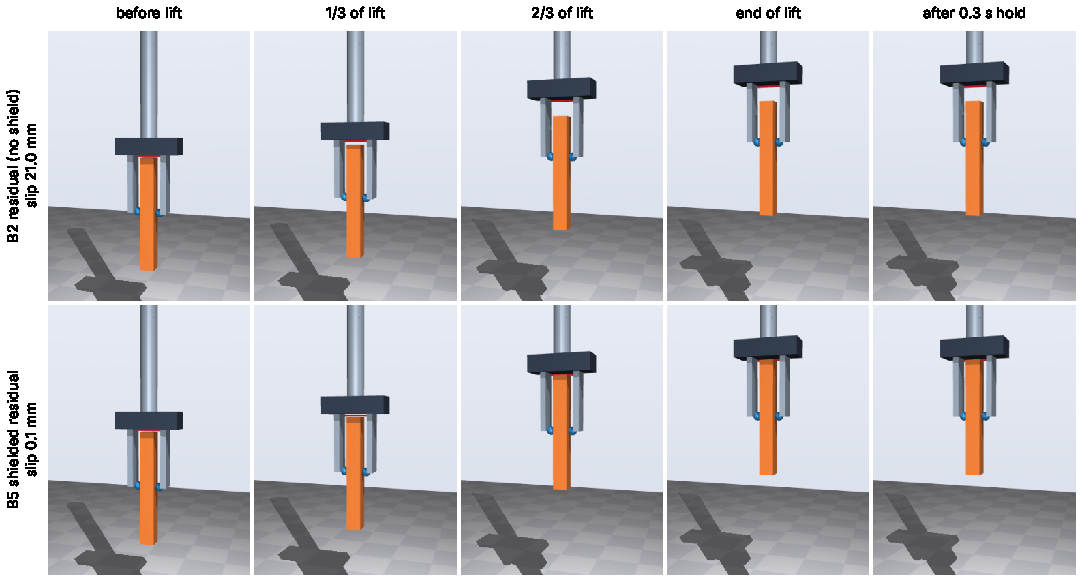
\includegraphics[width=\textwidth]{fig_render.pdf}
\caption{\textbf{One lift, two policies} (test object 2, 72\,g, $\mu_s=0.77$, $r=1.2$; MuJoCo renders replayed from the
recorded simulation states, with visual-only finger and palm geometry added). The red mark on the palm sits at the rod's
initial top. The unshielded residual (top) grips 9\% below the model's grip for its lift time; the rod breaks away near
peak acceleration and ends 21\,mm low. The shield-trained residual (bottom) lifts equally fast with a certified grip; the
rod does not move relative to the fingers.}\label{fig:render}
\end{figure*}

\finding{Rig.} We simulate the task in MuJoCo~3~\cite{todorov2012} at 1\,ms steps with elliptic friction cones, an
impedance ratio of 10 and 20 no-slip iterations. Two spherical pads (radius 6\,mm, torsional friction) close on a
2$\times$2$\times$16\,cm rod; each pad is driven by a force-controlled slide joint. The palm moves on a vertical slide joint
whose position and velocity are imposed at every step, so its acceleration follows the planned trajectory exactly. The
rod is constrained to a vertical slide: a free rod rocked about the grasp axis after slip and then crept, which mixes in a
pivoting motion we studied separately~\cite{aidoo2026a}; we study axial slip only. Appendix~\ref{app:sim} lists the model.

\finding{Stick--slip.} MuJoCo's contact model uses one friction coefficient. We emulate the drop from static to kinetic
friction as in~\cite{aidoo2026c}: the pads' friction switches from $\mu_s$ to $\mu_s/r$ when the rod's speed relative to the
fingers exceeds 2\,cm/s, and back below 2\,mm/s. We raised the switching thresholds during development, before any policy
was trained, because slow elastic creep at lower thresholds triggered kinetic friction on rods that were not slipping.

\begin{table}[t]\centering\footnotesize
\caption{\textbf{Rig validation} (development objects only, run before training).}\label{tab:val}
\setlength{\tabcolsep}{3pt}
\begin{tabular}{@{}lr@{}}\toprule
Check & Result\\\midrule
V1 static breakaway / $mg/(2\mu_s)$ ($n=20$) & 0.989 (0.986--1.014)\\
V2 lift breakaway / $m(g+a_{pk})/(2\mu_s)$:&\\
\quad $T=0.25$ / 0.35 / 0.5 / 1.0\,s ($n=8$ each) & 0.890 / 0.930 / 0.952 / 0.983\\
V3 random lifts, $r\sim U[1,1.2]$ ($n=120$):&\\
\quad slipped although bound was zero ($n=67$) & 0\\
\quad largest slip above its bound (creep) & 0.20\,mm\\
\quad held, non-zero bound: slip $<$ bound & 21 of 21\\
\quad dropped (bound $\ge$ 0.56\,m) & 32\\
\quad slip $>5$\,mm although bound $\le5$\,mm & 0\\
\quad probe slip, max; probes, median & 5.3\,mm; 8\\
V4 elastic creep, grip margin 1.1--2.0 & 0.09--0.19\,mm\\\bottomrule
\end{tabular}\end{table}

\finding{Validation.} Before training we checked the rig against the friction model (Table~\ref{tab:val}; details in
Appendix~\ref{app:val}). The static breakaway grip matched $mg/(2\mu_s)$ within 1.1\%. During lifts the grip at which the rod
broke away was 2--11\% below the quasi-static prediction $m(g+a_{pk})/(2\mu_s)$, more so for short lifts: the quasi-static
model is conservative, increasingly so as lifts get faster. We did not isolate the cause; contact compliance and the
short time the demand spends near its peak are candidates. In
120 lifts with random grips and durations, no rod slipped whose bound was zero (beyond 0.2\,mm of creep), every lift that kept the
rod slipped less than its non-zero bound (the 32 rods that were dropped all had bounds above half a metre, i.e.\ no
certificate at all), and no lift with a bound of at most 5\,mm slipped more than 5\,mm. Elastic creep in the pads, a stiff
spring rather than friction slip, moved the rod 0.1--0.2\,mm whatever the grip.

\section{Experimental Setup}\label{sec:setup}
\finding{Methods.} We compare six methods (Table~\ref{tab:methods}). B0 is the friction-model controller and B0S adds the
grip shield. B2 is a residual trained and tested without a shield. B4g and B4t apply the grip or time shield to B2's
commands at test time only; B5 is a residual trained and tested with the grip shield in the loop. Residuals were trained
with 5 seeds each on objects with $r\sim U[1.0,1.2]$, $r_{\max}=1.2$, for 1{,}560 episodes per run, starting from zero
weights, i.e.\ from the model controller.

\begin{table}[t]\centering\footnotesize
\caption{\textbf{Methods.}}\label{tab:methods}
\setlength{\tabcolsep}{3.5pt}
\begin{tabular}{@{}llcc@{}}\toprule
ID & Controller & Shield in training & Shield at test\\\midrule
B0 & friction model & -- & --\\
B0S & friction model & -- & grip\\
B2 & residual & no & no\\
B4g & residual (B2 weights) & no & grip\\
B4t & residual (B2 weights) & no & time\\
B5 & residual & grip & grip\\\bottomrule
\end{tabular}\end{table}

\finding{Evaluation sets.} The \emph{test set} has 40 new objects, each lifted at $r\in\{1.0,1.1,1.2,1.3\}$; $r=1.3$ lies
beyond the shield's assumed $r_{\max}=1.2$. Episode random seeds are shared across methods, so every method sees the same
weight-estimate error and sensor noise on each object. The \emph{confirmation set} has 40 further objects with
$r\sim U[1.0,1.3]$ per object and was run once, after the analysis code and the test-set results had been committed. For
\Q4 we also evaluate B0S and B5 with the shield set to $r_{\max}\in\{1.0,1.4\}$.

\finding{Questions.} \Q1: How much faster does a residual lift, and at what grip? \Q2: Does it stay safe as friction drops?
\Q3: Should the shield raise the grip or slow the lift? \Q4: Does the certificate hold, also when $r_{\max}$ is wrong, and
what does a slip allowance buy?

\finding{Metrics and statistics.} We report the failure count (slip $>5$\,mm or a drop) with Wilson 95\%
intervals~\cite{wilson1927}, the mean lift time $T$, the mean grip relative to the object's weight $F/mg$, and the largest
slip. Learned methods are averaged over the 5 seeds per object. We test lift time and grip against B0 with paired
Wilcoxon signed-rank tests over objects~\cite{wilcoxon1945}, and per-object failures with exact McNemar
tests~\cite{mcnemar1947}, Holm-corrected within each question~\cite{holm1979}; mean differences carry hierarchical
bootstrap 95\% intervals that resample seeds, then objects~\cite{efron1993}.

\finding{Pre-registration.} The task, rig, questions, methods, sets, metrics and tests were committed to the repository
before any policy was trained~\cite{nosek2018}. Three dated deviations are recorded there (Section~\ref{sec:lim}). The
controlled study, safety map, bound-tightness and trace analyses of Section~\ref{sec:extended} were designed after the
confirmatory results were known; they were frozen in a protocol addendum before they were run and are reported as
exploratory.
